\documentclass[a4paper, 12pt]{article}%тип документа

%отступы
\usepackage[left=2cm,right=2cm,top=2cm,bottom=3cm,bindingoffset=0cm]{geometry}

%Русский язык
\usepackage[T2A]{fontenc} %кодировка
\usepackage[utf8]{inputenc} %кодировка исходного кода
\usepackage[english,russian]{babel} %локализация и переносы

%Вставка картинок
\usepackage{wrapfig}
\usepackage{graphicx}
\graphicspath{{pictures/}}
\DeclareGraphicsExtensions{.pdf,.png,.jpg}

%Графики
\usepackage{multirow}
\usepackage{pgfplots}
\pgfplotsset{compat=1.9}

%Математика
\usepackage{amsmath, amsfonts, amssymb, amsthm, mathtools}

%Заголовок
\author{Валеев Рауф Раушанович \\
группа 825}
\title{\textbf{Работа 2.1.3 \\ 
Определение $C_p / C_v$ по скорости звука в газе}}
\begin{document}
\maketitle
\newpage
\section*{Цель работы}
\begin{enumerate}
\item измерение частоты колебаний и длины волны при резонансе звуковых колебаний в газе, заполняющем трубу
\item определение показателя адиабаты с помощью уравнения состояния идеального газа
\end{enumerate}
\section*{Краткая теоретическая справка}
\subsection*{Скорость звука}
Распространение звуковой волны в газе происходит адиабатически. Сжатия и разрежения в газе сменяют друг друга настолько быстро, что теплообмен между слоями газа, имеющими разные температуры, не успевает произойти. Используя полученное уравнение адиабаты идеального газа, найдем скорость звука по общей формуле
\[c = \sqrt{\dfrac{dP}{d \rho}}\]
Заменим в уравнение Пуассона $PV^{\gamma} = const$ объем на плотность $\rho = \dfrac{m}{V}$, после чего получим $P = const \cdot \rho^{\gamma}$. Тогда после логарифмирования и дифференцирования этого выражения имеем 
\[ \dfrac{dP}{P} = \gamma \dfrac{d \rho }{\rho} \text{, или } \left( \dfrac{dP}{d\rho} \right)_\text{адиабат} = \sigma \dfrac{P}{\rho} \]
откуда для скорости звука получаем.
\[ c = \sqrt{\left( \dfrac{dP}{d\rho} \right)_\text{адиабат}} = \sqrt{\gamma \dfrac{P}{\rho}} = // PV = \dfrac{\mu}{m} RT // = \sqrt{\gamma \dfrac{RT}{\mu}} \Rightarrow \]
\[ \gamma = \dfrac{\mu}{RT} c^2\]
Таким образом, для определения показателя адиабаты достаточно измерить температуру газа и скорость распространения звука (молярная масса газа предполагается известной).

Звуковая волна, распространяющаяся вдоль трубы, испытывает многократное отражение от торцов. Звуковые колебания в трубе являются наложением всех отраженных волн и, вообще говоря, очень сложны. Картина упрощается, если длина трубы $L$ равна целому числу полуволн, то есть когда 
\[L = n \dfrac{\lambda}{2}\]
\[c = \lambda f\]
Подбор условий, при которых возникает резонанс, можно производить двояко:
\begin{enumerate}
\item При неизменной частоте $f$ звукового генератора (а, следовательно, и неизменной длине звуковой волны $\lambda$) можно измерять длину трубы $L$.
\item При постоянной длине трубы можно изменять частоту звуковых колебаний. В этом случае следует плавно изменять частоту $f$ звукого генератора, а следовательно, и длину звуковой волны $\lambda$. Для последовательных резонансов получим 
\[L = \dfrac{\lambda_1}{2}n = \dfrac{\lambda_2}{2}(n+1) = ... = \dfrac{\lambda_{k+1}}{2}(n+k)\]
Отсюда имеем, что 
\[f_1 = \dfrac{c}{\lambda_1} = \dfrac{c}{2L}n, \text{ } f_2 = \dfrac{c}{\lambda_2} = \dfrac{c}{2L}(n+1) = f_1 +  \dfrac{c}{2L},...,\]
\[f_{k+1} = \dfrac{c}{\lambda_{k+1}} = \dfrac{c}{2L}(n+k) = f_1 +  \dfrac{c}{2L}k\]  
\end{enumerate}
\subsection*{Экспериментальная установка}
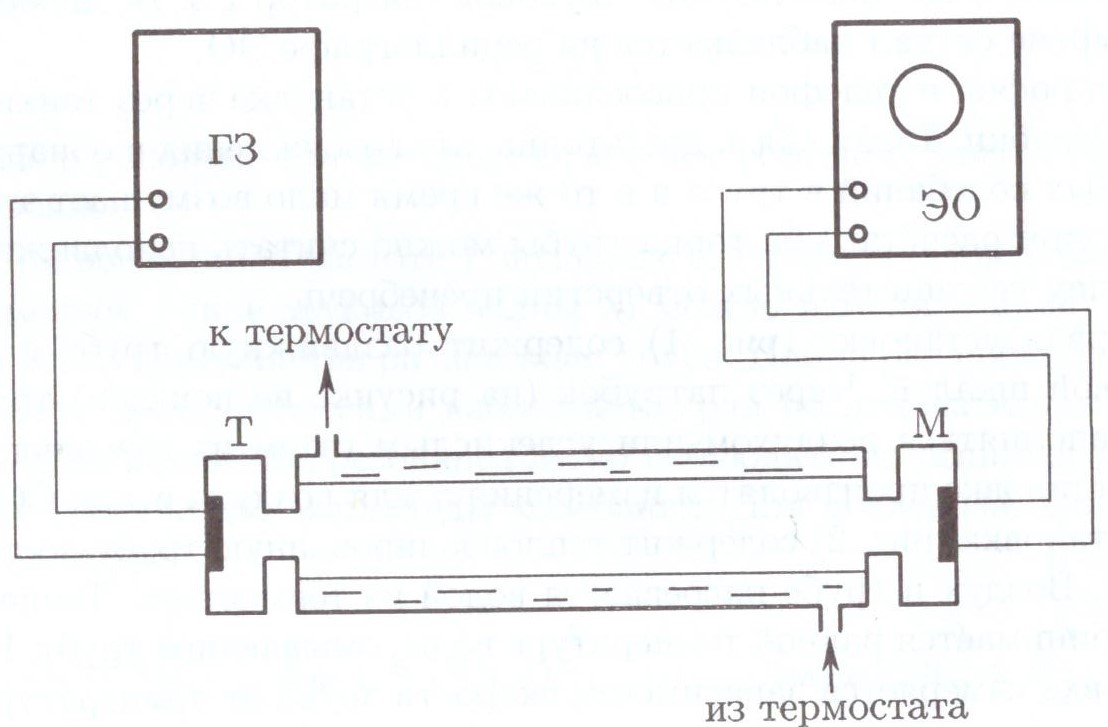
\includegraphics[width = 0.9\textwidth]{213_1.jpg}

Здесь звуковые колебания возубждаются телефоном Т и улавливаются микрофоном М. Мембрана телефона приводится в движение переменным током звуковой частоты; в качестве источника переменной ЭДС используется звуковой генератор ГЗ. Возникающей в микрофоне сигнал наблюдается на осцилографе ЭО.

Микрофон и телефон подсоединены к установке через тонкие резиновые трубки. Такая связь достаточна для возбуждения и обнаружения звуковых колебаний в трубе и в то же время мало возмущает эти колебания.

Установка содержит теплоизолированную трубу постоянной длины. Воздух в трубе нагревается из термостата. Температура газа принимается равной температуре воды, омывающей трубу.  
\section*{Ход работы}
\begin{enumerate}
\item  ЭО и ЗГ для дальнейшей работы.
\item Измеряем скорость звука в трубе постоянной длины. Плавно увеличивая частоту генератора, получаем ряд последовательных резонансных значений частоты, отмечая момент резонанса по увеличению амплитуды колебаний на экране осцилогрофа.
\item Строим график, откладывая по оси абсцисс номер резонанса $k$, а по оси ординат - $f_{k+1} - f_1$. Угловой коэффициент прямой определяет велечину $c / 2L$, где $L = (740 \pm 1)$ мм.
\item Повторяем 2 и 3 для разных температур.\\
\begin{tabular}{|c|c|c|}
\hline
\multicolumn{3}{|c|}{$T = (24,2 \pm 0,1) ^{\circ}C$} \\ \hline
Номер & $f, kHz$ & $\sigma_f, kHz$ \\ \hline
1 & 1,16 & 0,01 \\ \hline
2 & 1,39 & 0,01 \\ \hline
3 & 1,62 & 0,01 \\ \hline
4 & 1,86 & 0,01 \\ \hline
5 & 2,07 & 0,01 \\ \hline
6 & 2,31 & 0,01 \\ \hline
7 & 2,55 & 0,01 \\ \hline
8 & 2,78 & 0,01 \\ \hline
9 & 3,00 & 0,01 \\ \hline
\end{tabular}
\begin{tabular}{|c|c|c|}
\hline
\multicolumn{3}{|c|}{$T = (35 \pm 0,1) ^{\circ}C$} \\ \hline
Номер & $f, kHz$ & $\sigma_f, kHz$ \\ \hline
1 & 0,71 & 0,01 \\ \hline
2 & 0,95 & 0,01 \\ \hline
3 & 1,19 & 0,01 \\ \hline
4 & 1,41 & 0,01 \\ \hline
5 & 1,65 & 0,01 \\ \hline
6 & 1,89 & 0,01 \\ \hline
7 & 2,13 & 0,01 \\ \hline
8 & 2,36 & 0,01 \\ \hline
9 & 2,59 & 0,01 \\ \hline
10 & 2,83 & 0,01 \\ \hline
\end{tabular}
\begin{tabular}{|c|c|c|}
\hline
\multicolumn{3}{|c|}{$T = (45 \pm 0,1) ^{\circ}C$} \\ \hline
Номер & $f, kHz$ & $\sigma_f, kHz$ \\ \hline
1 & 0,73 & 0,01 \\ \hline
2 & 0,96 & 0,01 \\ \hline
3 & 1,21 & 0,01 \\ \hline
4 & 1,45 & 0,01 \\ \hline
5 & 1,68 & 0,01 \\ \hline
6 & 1,92 & 0,01 \\ \hline
7 & 2,16 & 0,01 \\ \hline
8 & 2,39 & 0,01 \\ \hline
9 & 2,63 & 0,01 \\ \hline
10 & 2,89 & 0,01 \\ \hline
\end{tabular}

\begin{tabular}{|c|c|c|}
\hline
\multicolumn{3}{|c|}{$T = (55 \pm 0,1) ^{\circ}C$} \\ \hline
Номер & $f, kHz$ & $\sigma_f, kHz$ \\ \hline
1 & 0,75 & 0,01 \\ \hline
2 & 0,99 & 0,01 \\ \hline
3 & 1,23 & 0,01 \\ \hline
4 & 1,46 & 0,01 \\ \hline
5 & 1,7 & 0,01 \\ \hline
6 & 1,95 & 0,01 \\ \hline
7 & 2,19 & 0,01 \\ \hline
8 & 2,43 & 0,01 \\ \hline
9 & 2,68 & 0,01 \\ \hline
10 & 2,93 & 0,01 \\ \hline
\end{tabular}
\begin{tabular}{|c|c|c|}
\hline
\multicolumn{3}{|c|}{$T = (60 \pm 0,1) ^{\circ}C$} \\ \hline
Номер & $f, kHz$ & $\sigma_f, kHz$ \\ \hline
1 & 0,74 & 0,01 \\ \hline
2 & 0,99 & 0,01 \\ \hline
3 & 1,23 & 0,01 \\ \hline
4 & 1,48 & 0,01 \\ \hline
5 & 1,71 & 0,01 \\ \hline
6 & 1,97 & 0,01 \\ \hline
7 & 2,21 & 0,01 \\ \hline
8 & 2,45 & 0,01 \\ \hline
9 & 2,7 & 0,01 \\ \hline
10 & 2,96 & 0,01 \\ \hline
\end{tabular}

\begin{tabular}{|c|c|c|c|c|}
\hline
$T, ^{\circ}C$ & $c$ м/c & $\sigma_c$, м/c & $\gamma$ & $\sigma_{\gamma}$ \\ \hline
24,2 & 341 & 1,3 & 1,368 & 0,009 \\ \hline
35 & 348 & 1,3 & 1,372 & 0,008 \\ \hline
45 & 353 & 1,3 & 1,370 & 0,008 \\ \hline
55 & 359 & 1,3 & 1,368 & 0,007 \\ \hline
60 & 363 & 1,3 & 1,377 & 0,007 \\ \hline
\end{tabular}
\begin{figure}
\begin{wrapfigure}{r}{\textwidth}
  \begin{center}
    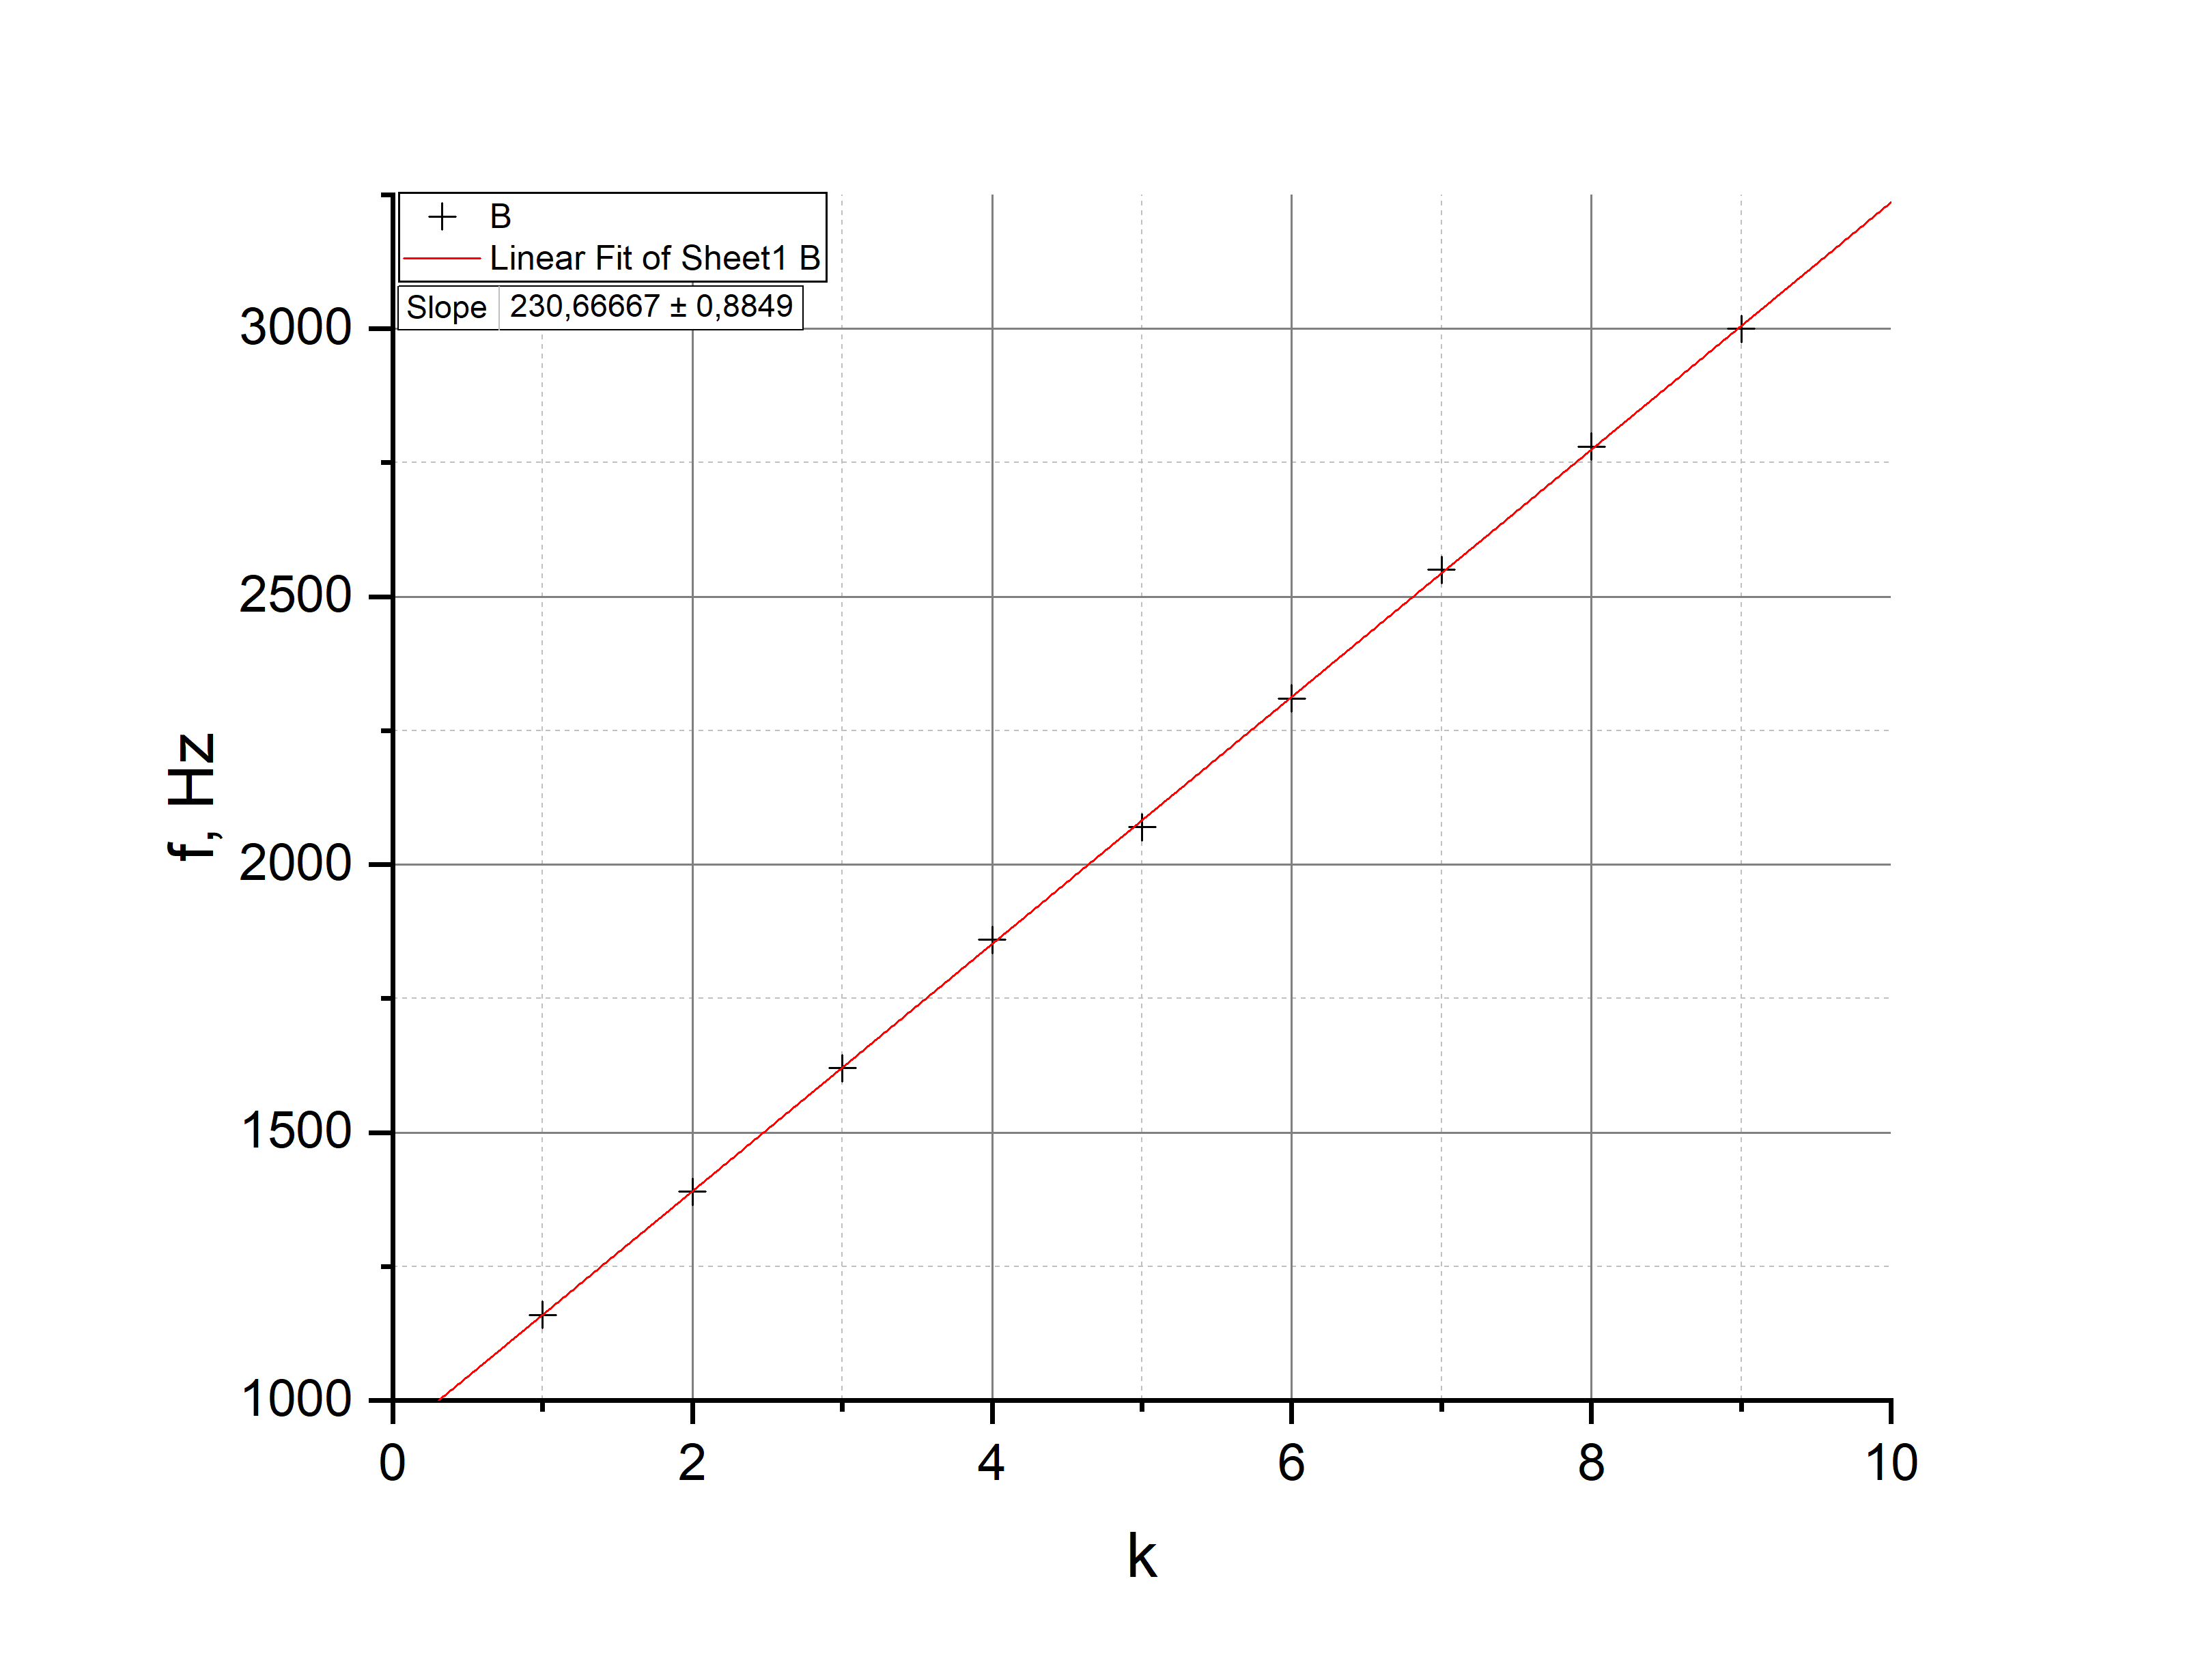
\includegraphics[width = \textwidth]{213_2.jpg}
  \end{center}
  \textbf{\caption{$T = (24,2 \pm 0,1) ^{\circ}C$}}
\end{wrapfigure}
\end{figure}
\begin{figure}
\begin{wrapfigure}{r}{\textwidth}
  \begin{center}
    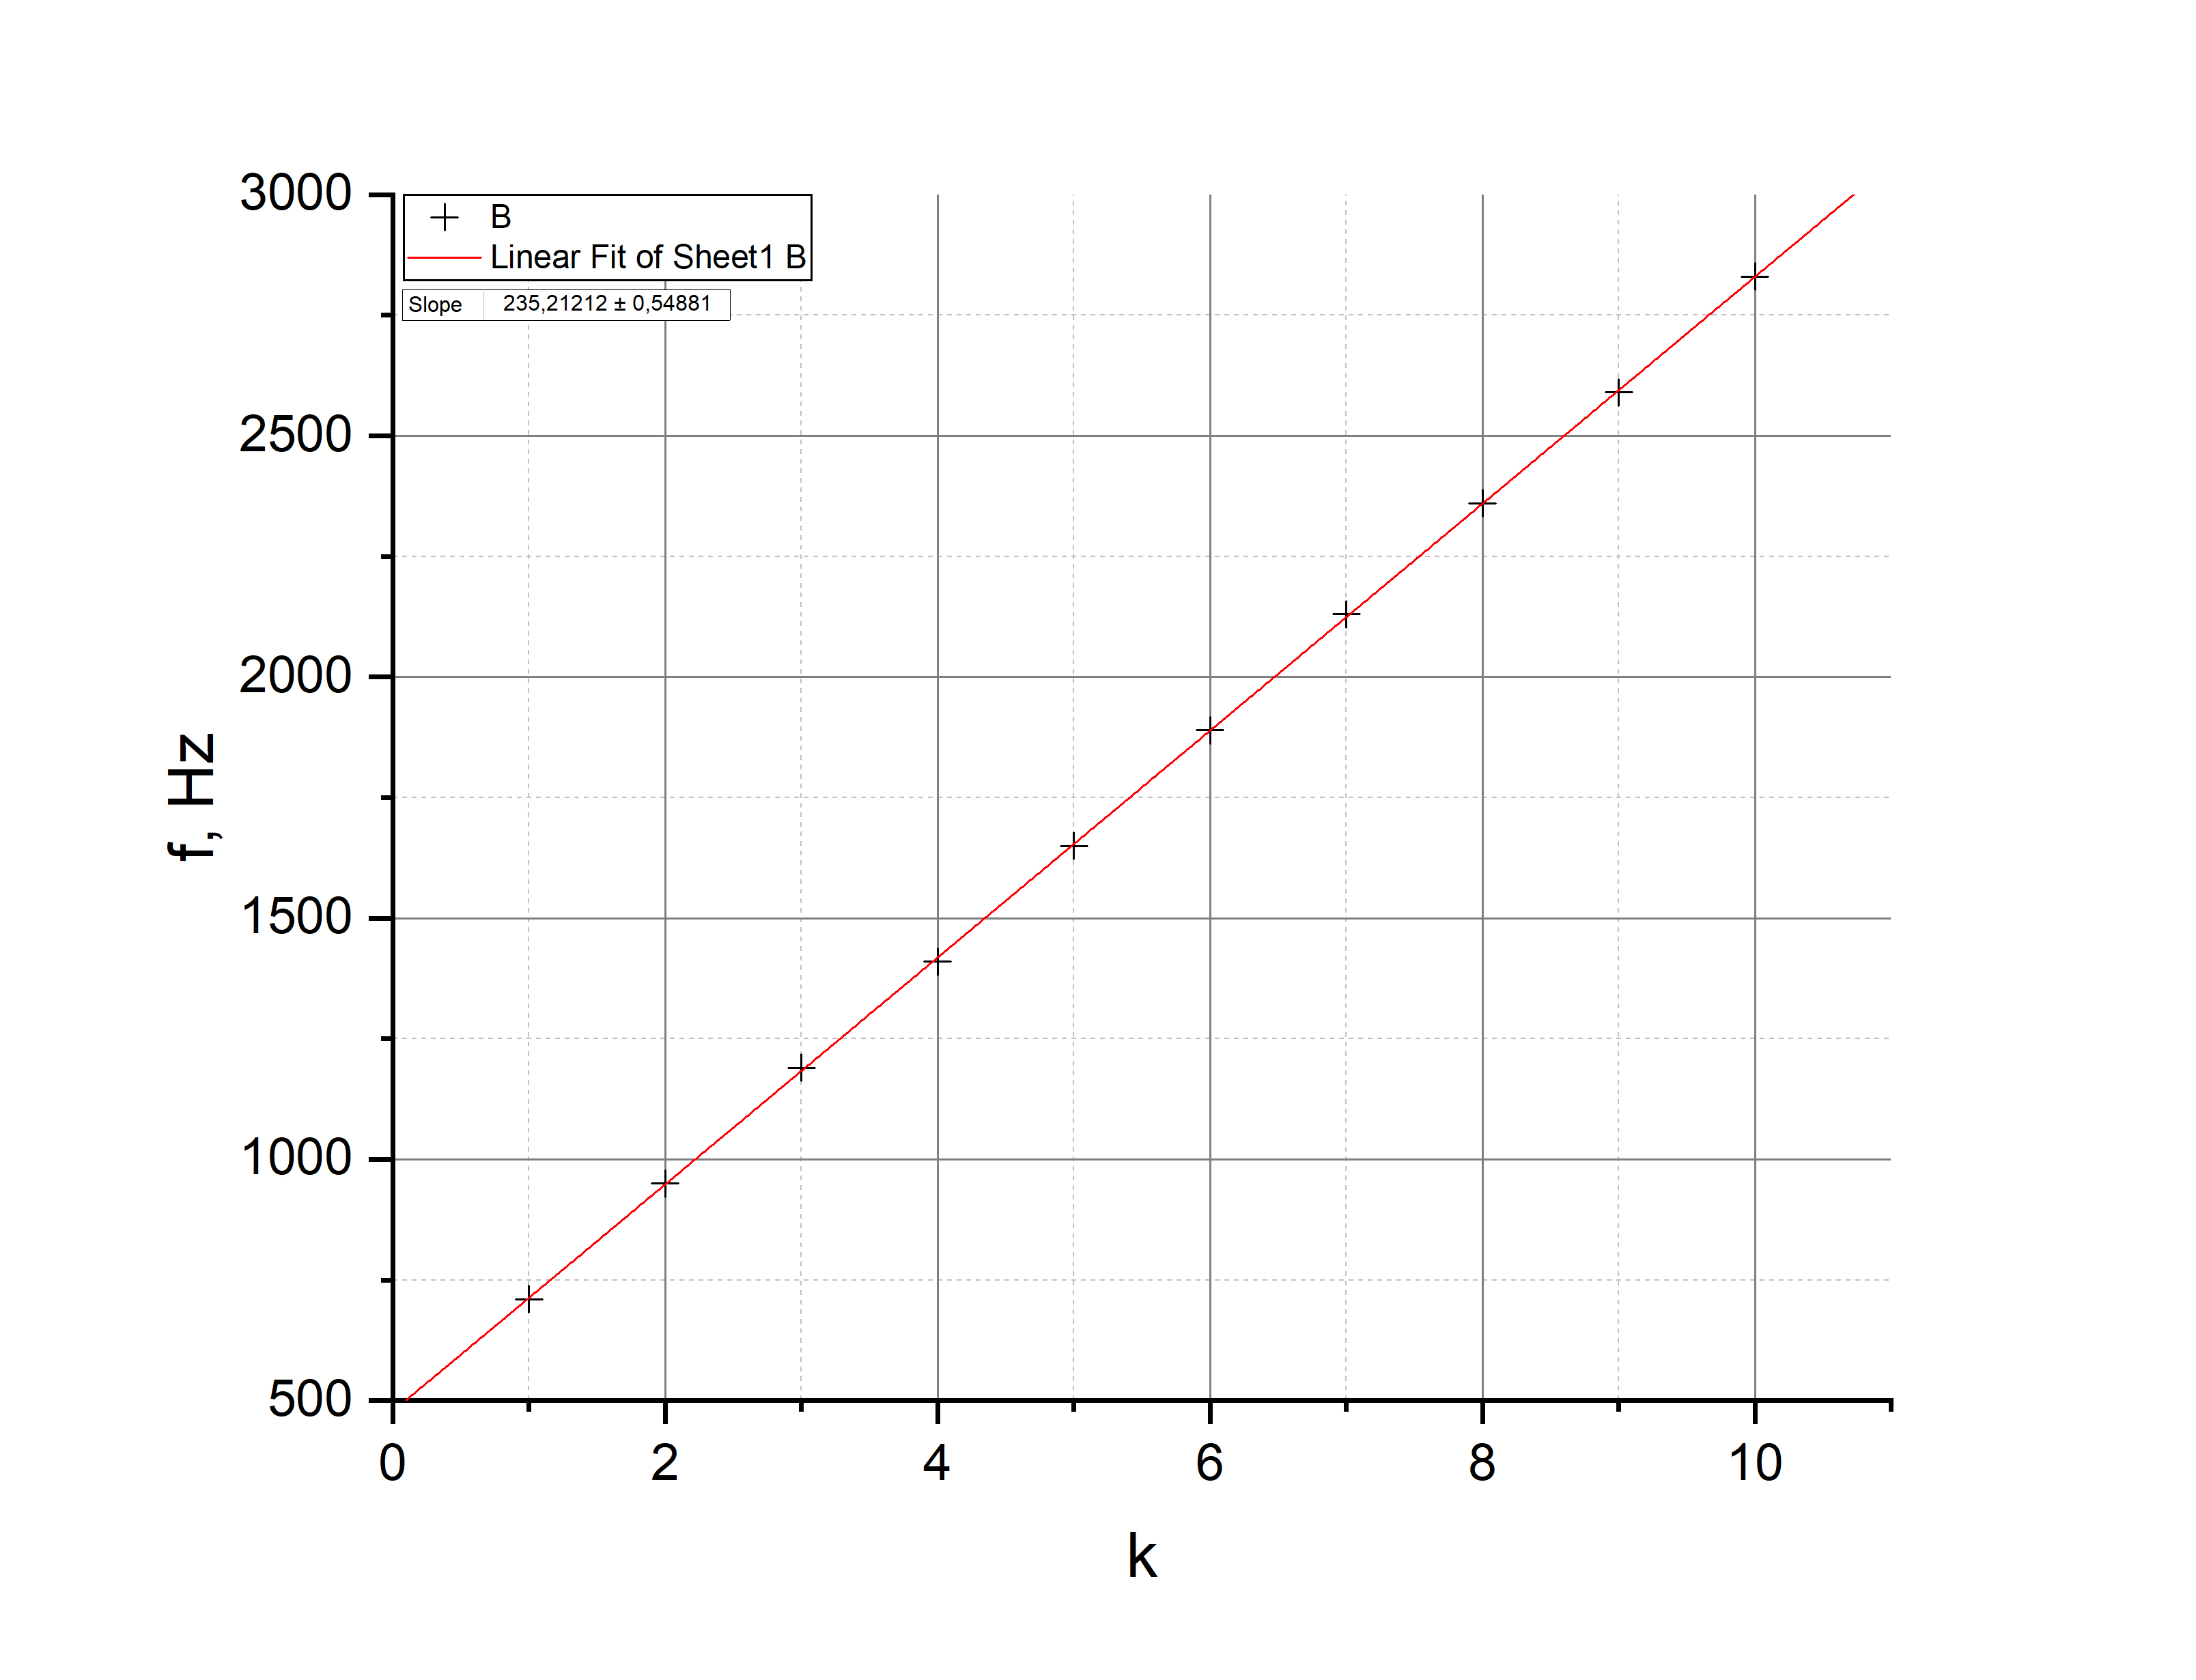
\includegraphics[width = \textwidth]{213_3.jpg}
  \end{center}
  \textbf{\caption{$T = (35 \pm 0,1) ^{\circ}C$}}
\end{wrapfigure}
\end{figure}
\begin{figure}
\begin{wrapfigure}{r}{\textwidth}
  \begin{center}
    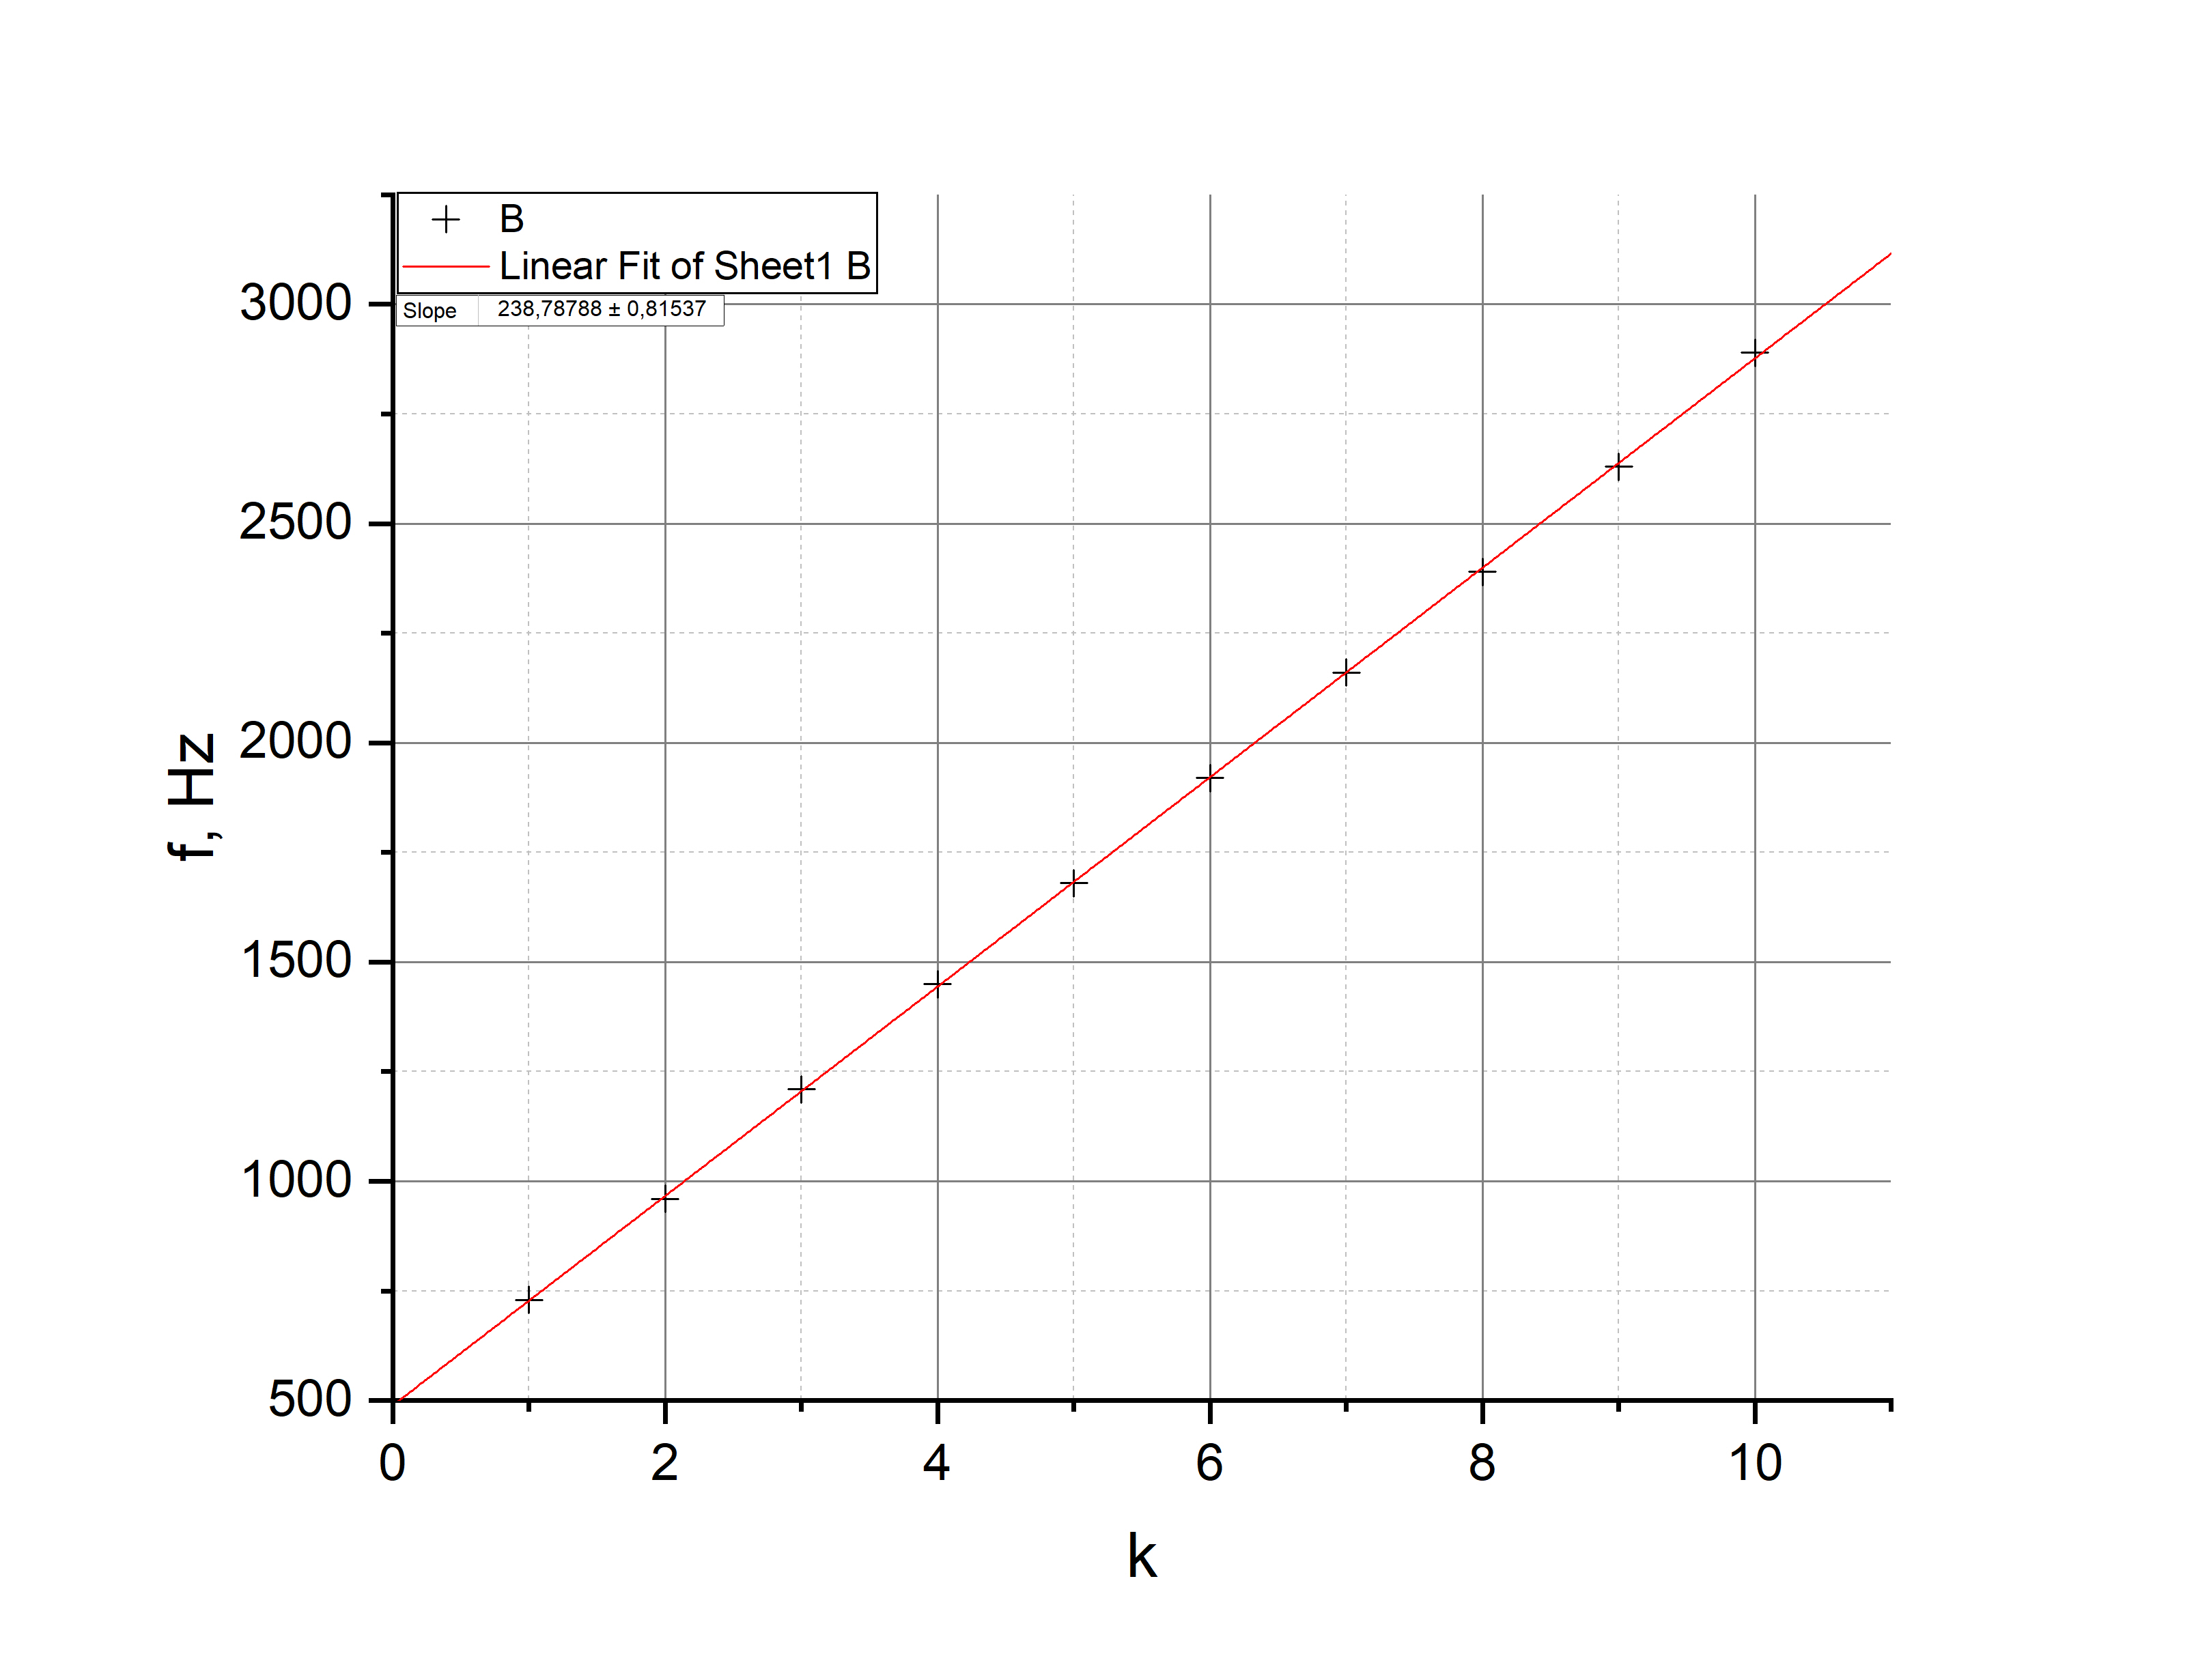
\includegraphics[width = \textwidth]{213_4.jpg}
  \end{center}
  \textbf{\caption{$T = (45 \pm 0,1) ^{\circ}C$}}
\end{wrapfigure}
\end{figure}
\begin{figure}
\begin{wrapfigure}{r}{\textwidth}
  \begin{center}
    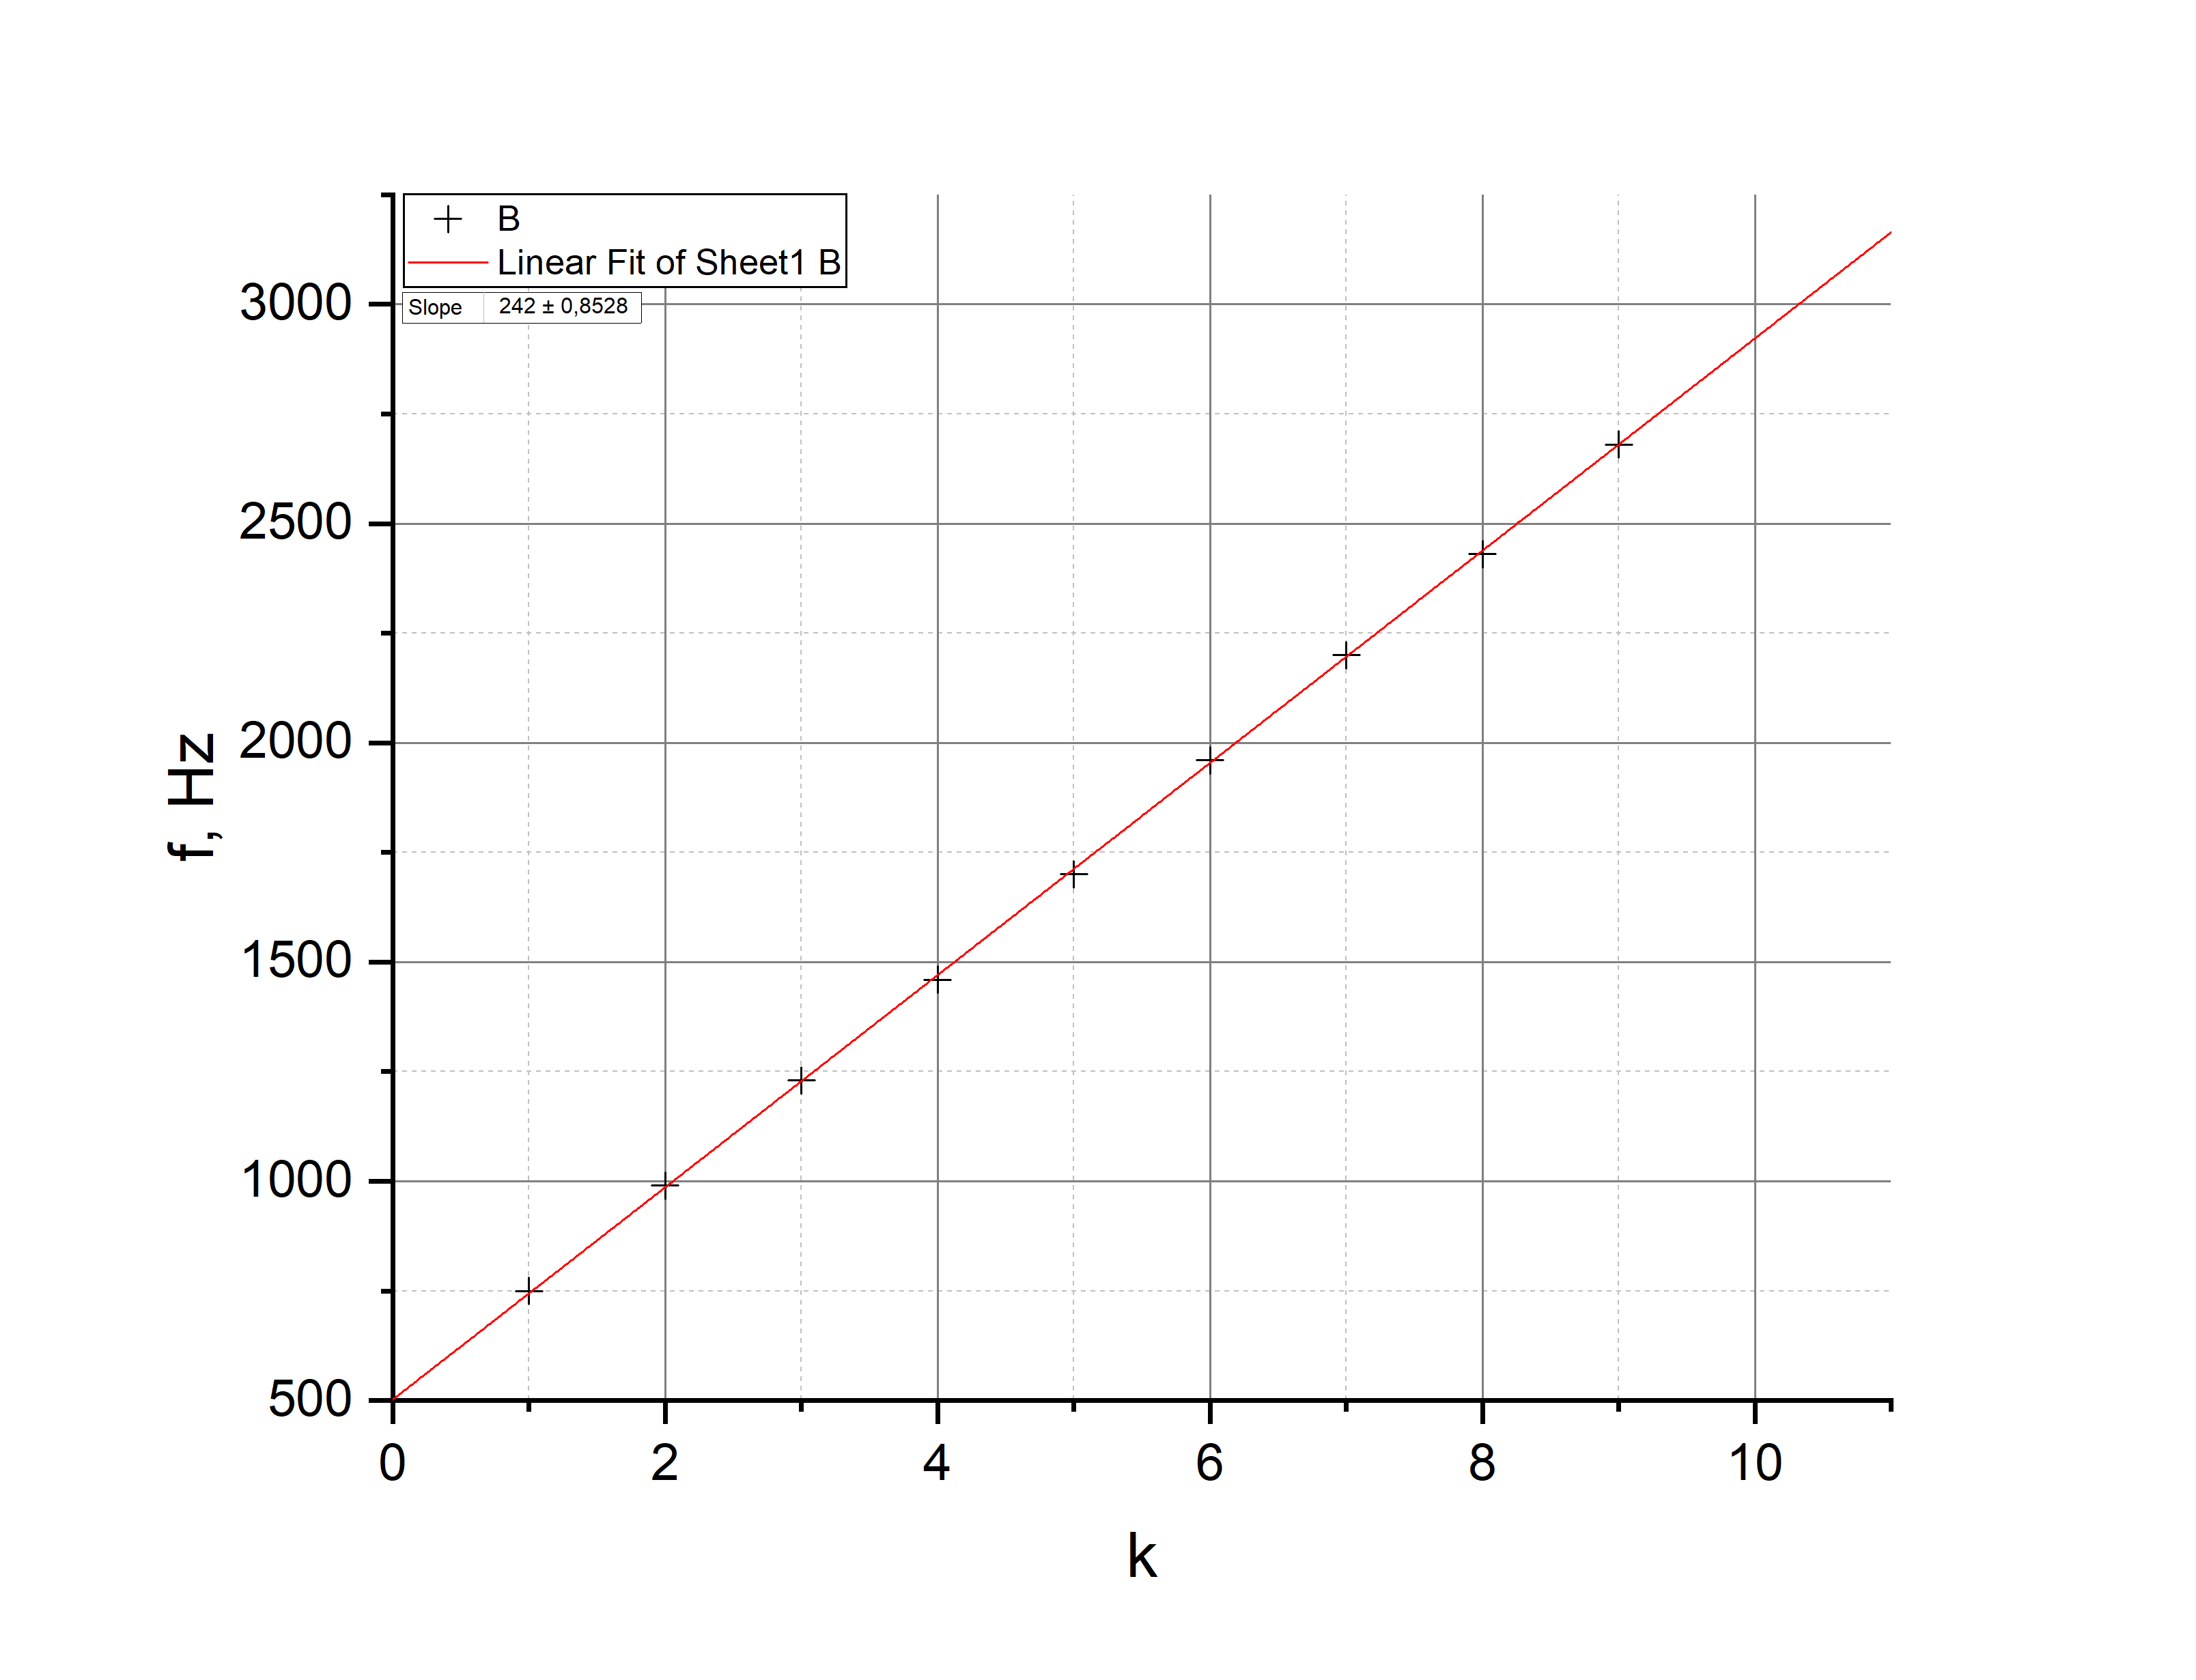
\includegraphics[width = \textwidth]{213_5.jpg}
  \end{center}
  \textbf{\caption{$T = (55 \pm 0,1) ^{\circ}C$}}
\end{wrapfigure}
\end{figure}
\begin{figure}
\begin{wrapfigure}{r}{\textwidth}
  \begin{center}
    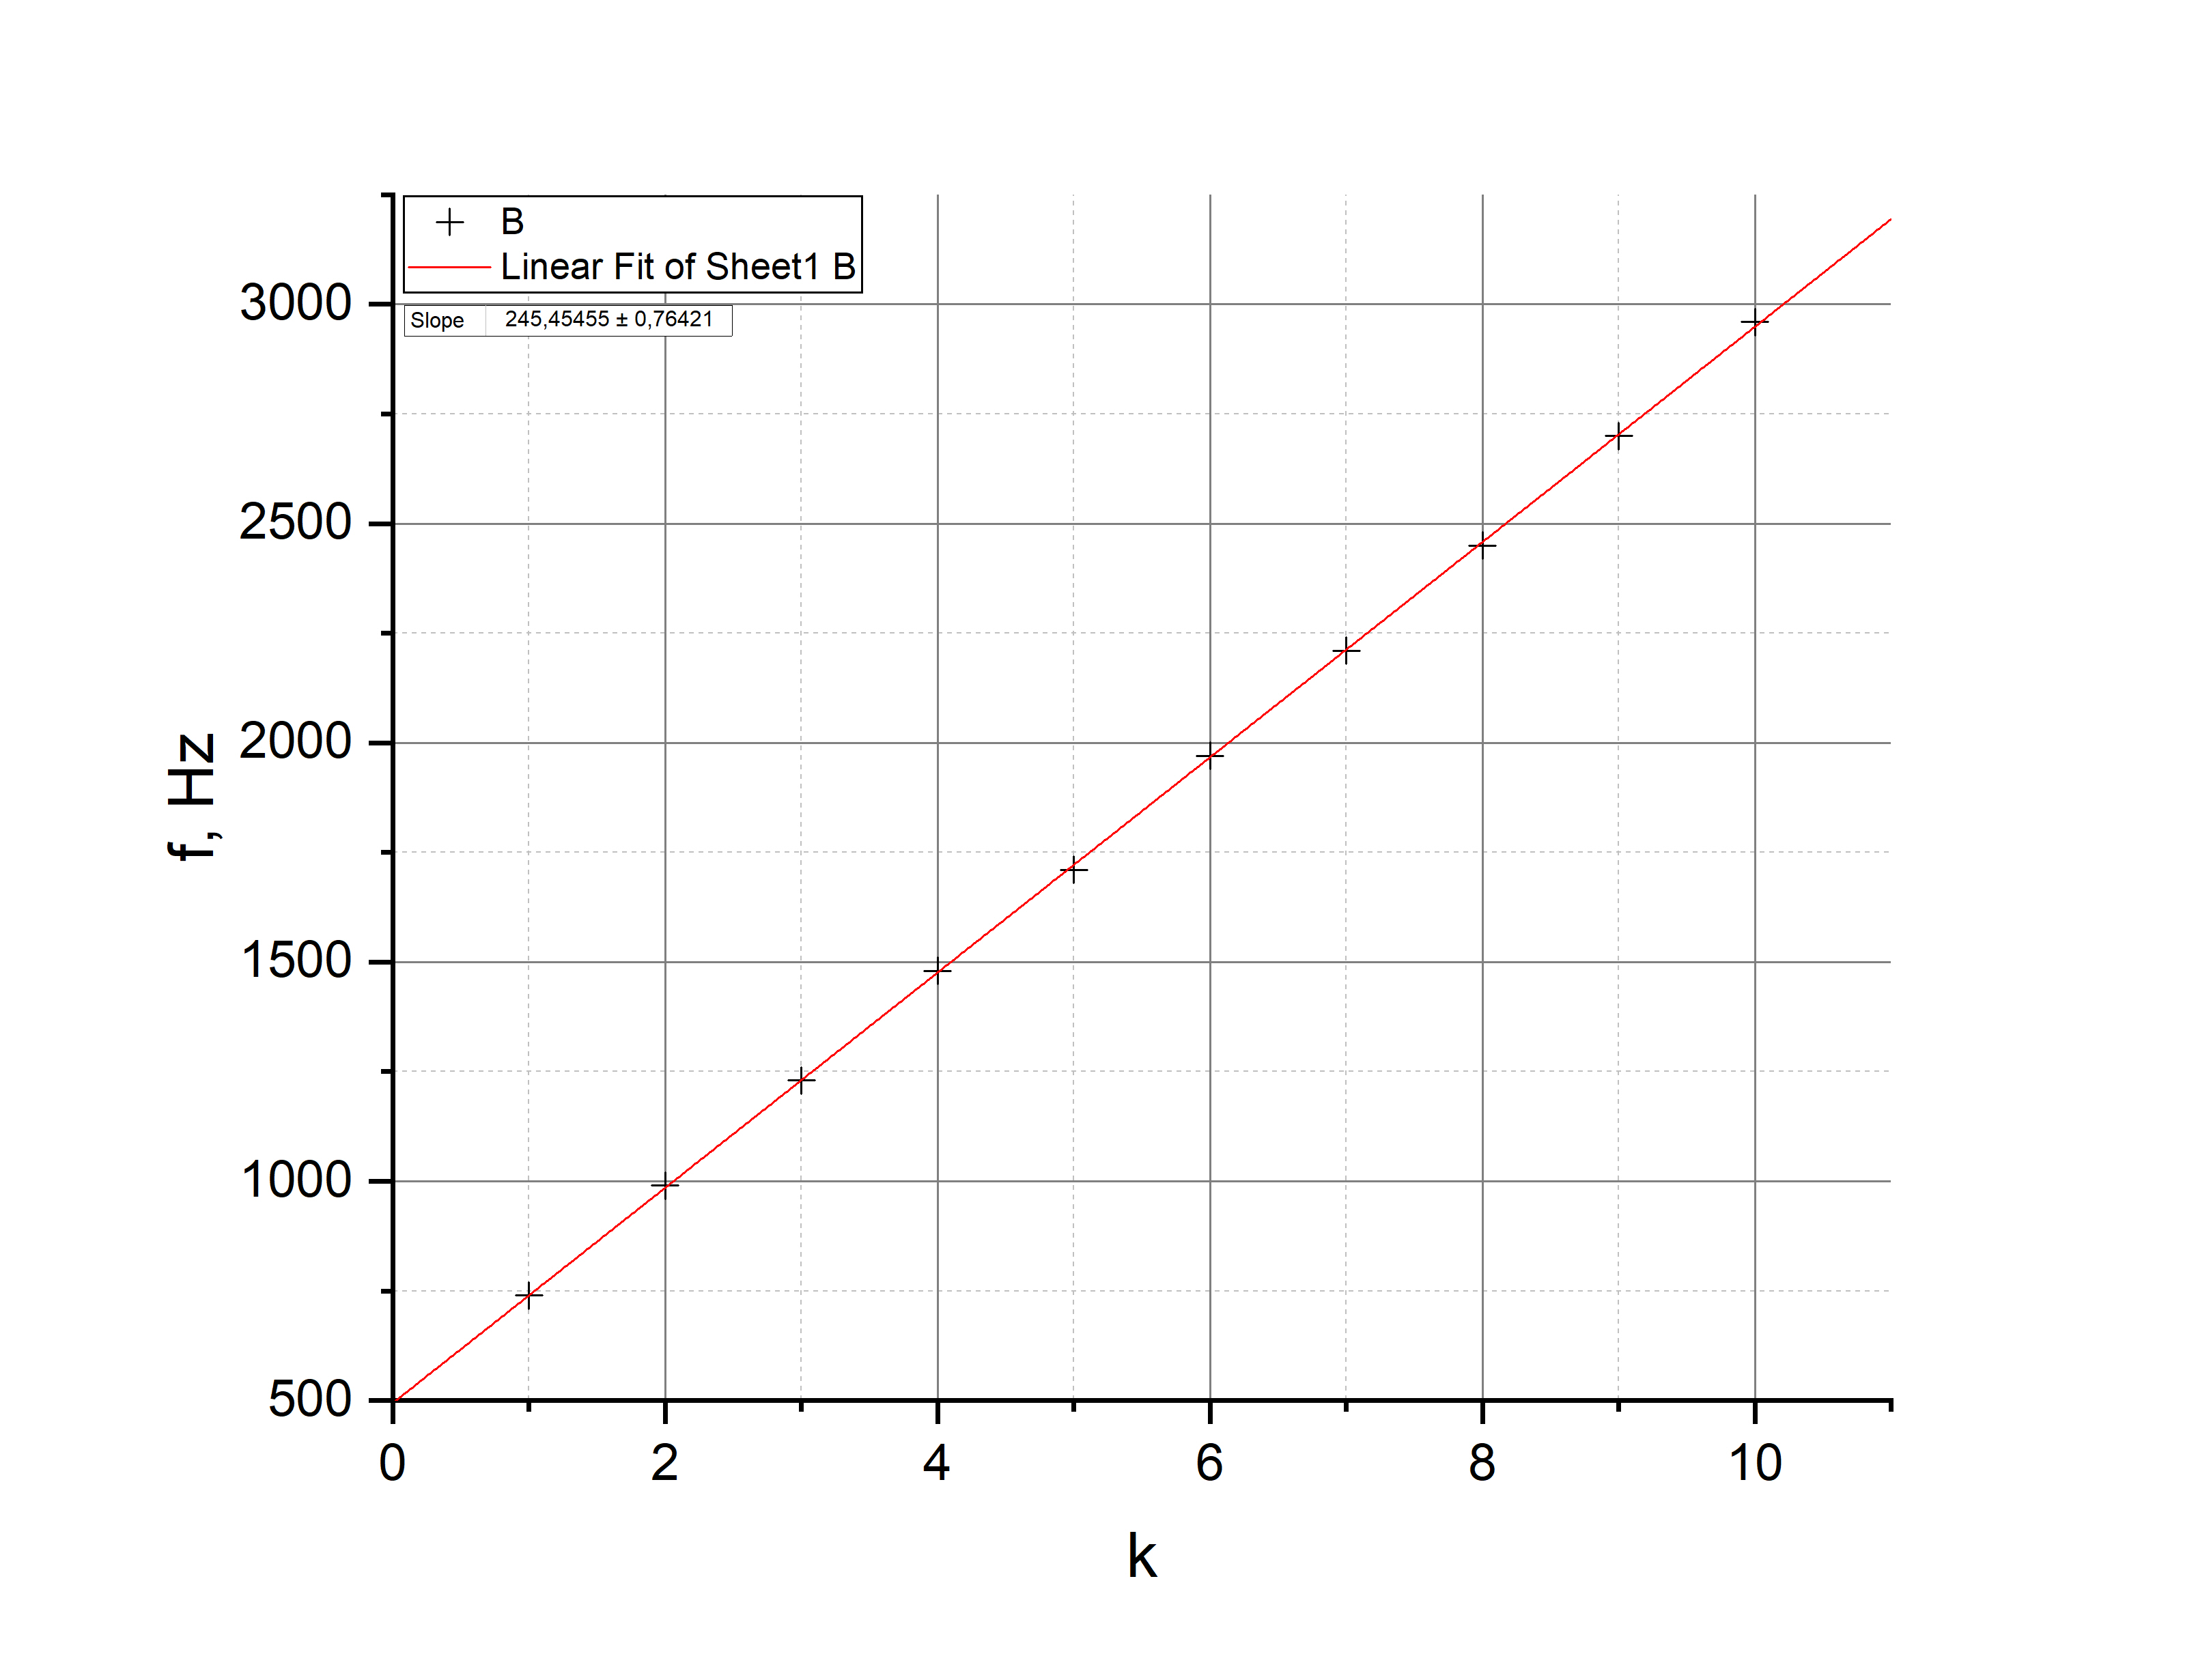
\includegraphics[width = \textwidth]{213_6.jpg}
  \end{center}
  \textbf{\caption{$T = (60 \pm 0,1) ^{\circ}C$}}
\end{wrapfigure}
\end{figure}

\item Вычисляем значение $\gamma = C_p / C_v$.
\end{enumerate}
\end{document}